\documentclass{article}
\usepackage{polski}
\usepackage[utf8]{inputenc}
\usepackage{natbib}
\usepackage{graphicx}
\usepackage{xcolor}
\usepackage{mathtools}
\usepackage{amssymb}
\usepackage[makeroom]{cancel}
\usepackage{hyperref}


\title{Sprawozdanie 4}
\author{Jan Bronicki}
\date{}


\begin{document}

\maketitle

\section{Cel ćwiczenia}

Cel ćwiczenia to obliczenie parametrów, przeprowadzenie symulacji oraz wyznaczenie wykresów charakteryzujączych układy sterowania NPN i PNP (0-20 mA).

Dobrane 3 różne wartości $R_{pom}$ to $\Omega, \Omega, \Omega$.
Rezystancja obiciążenie $R_{obc}=\Omega$.

\section{Moduł 0-20mA, Tranzystor NPN}

\subsection{$R_{pom}$}

Napięcia do sterowania:\\
$U_{pom, 0mA}=mA\cdot 10\Omega=0.04V$\\
$U_{pom, 20mA}=mA\cdot 10\Omega=0.2V$


Dobranie rezystorów (prað $I_{1}=4mA$):

$$
    R_{1}=\frac{23.8V}{4mA}=5.95k\Omega
$$

$$
    R_{2}=\frac{0.04V}{4mA}=10\Omega
$$


$$
    R_{ptm}=\frac{0.16V}{4mA}=40\Omega
$$


Maksymalne wartości rezystancji obciążenie:

$$
    R_{MAX, 4mA}=\frac{24V-0.1V-0.04V}{4mA}=5965\Omega
$$

$$
    R_{MAX, 20mA}=\frac{24V-0.1V-0.2V}{20mA}=1193\Omega
$$

\newpage

\begin{figure}[h!]
    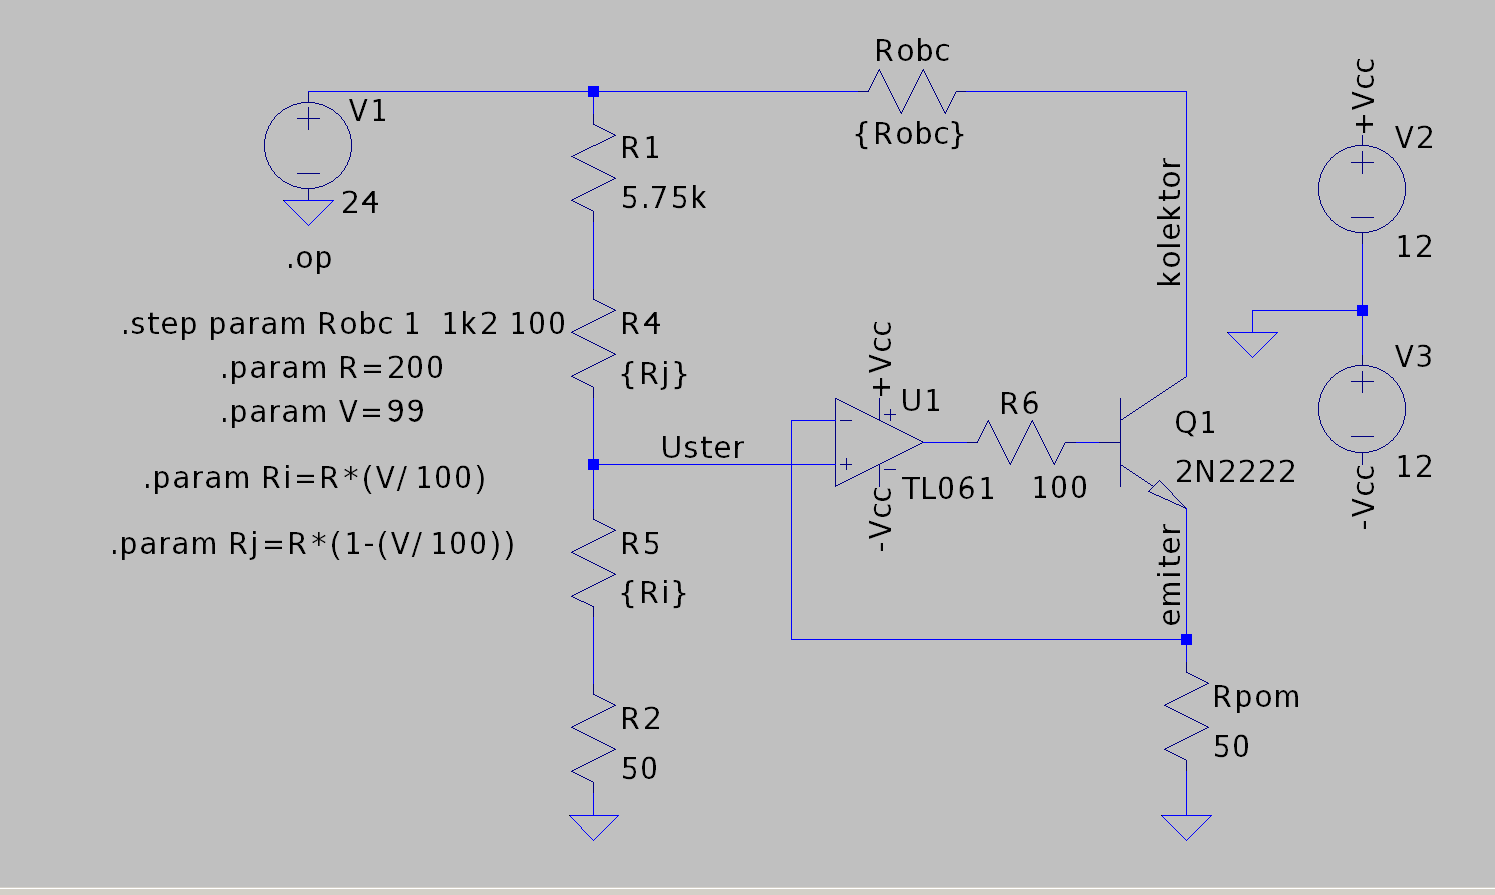
\includegraphics[scale=0.2]{schemat1.png}
    \centering
    \caption{Schemat NPN}
\end{figure}

\begin{figure}[h!]
    \centering
    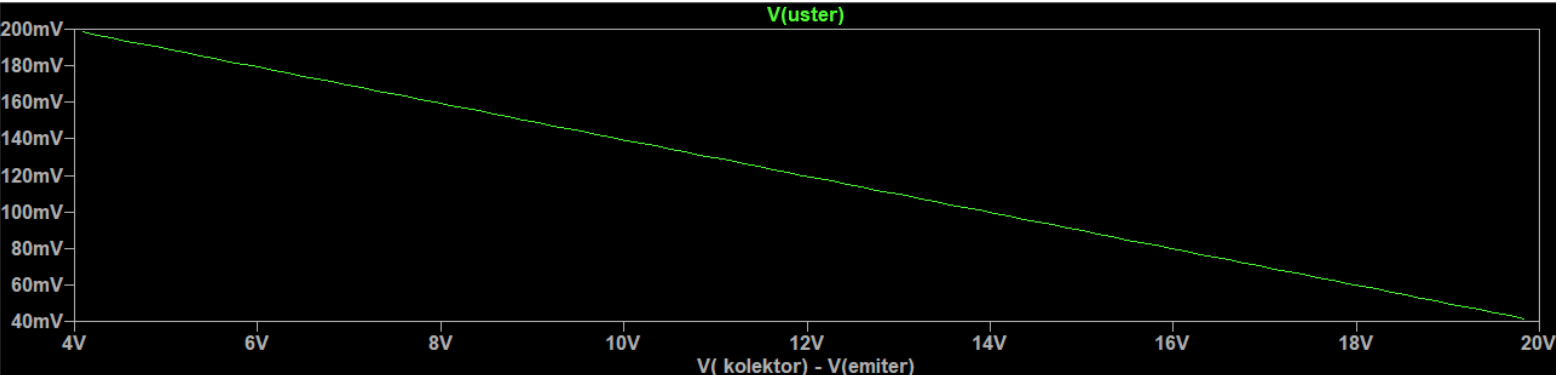
\includegraphics[scale=0.3]{p1.png}
    \caption{$U_{ster}(U_{ce})$}
\end{figure}


\begin{figure}[h!]
    \centering
    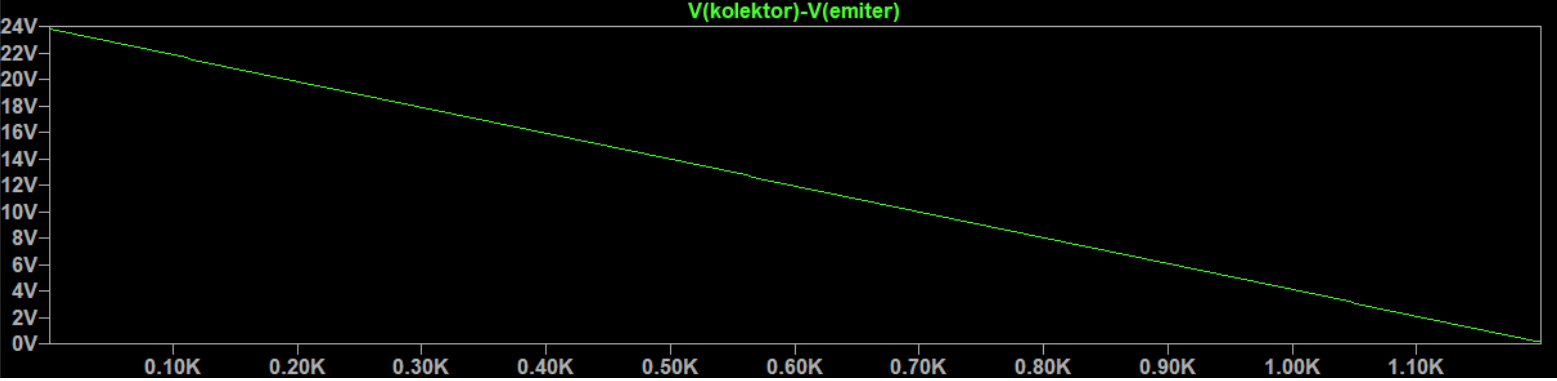
\includegraphics[scale=0.3]{p2.png}
    \caption{$U_{ce}(R_{obc}$)}
\end{figure}


\begin{figure}[h!]
    \centering
    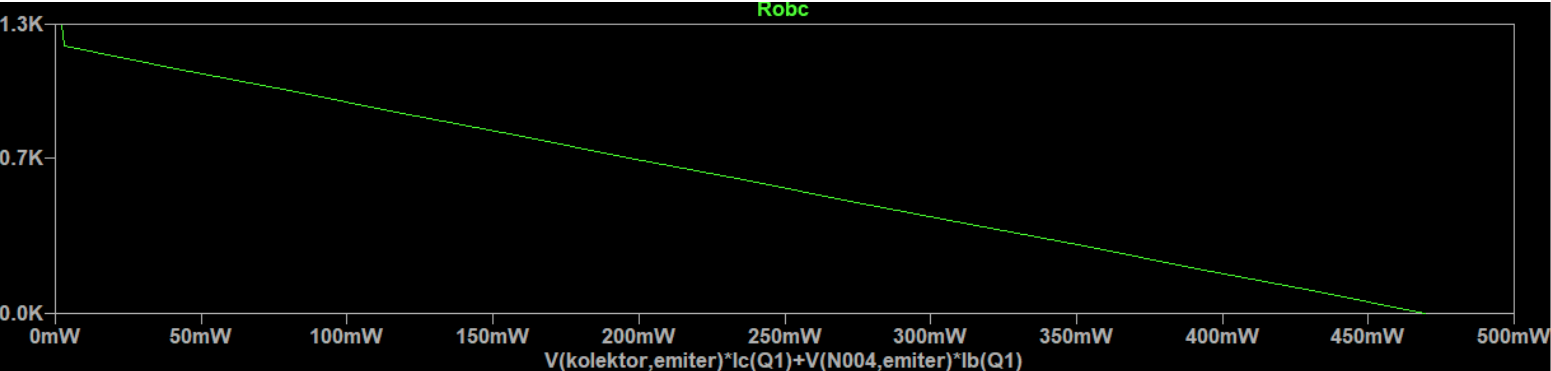
\includegraphics[scale=0.3]{p3.png}
    \caption{$R_{obc}(P_{diss})$}
\end{figure}

\subsection{$R_{pom}=50\Omega$}

Napięcia sterujące układem:\\
$U_{pom, 4mA}=4mA\cdot 50\Omega=0.2V$\\
$U_{pom, 20mA}=20mA\cdot 50\Omega=1V$


Dobranie rezystorów (przyjmuję prąd $I_{1}=4mA$):

$$
    R_{1}=\frac{23V}{4mA}=5.75k\Omega
$$

$$
    R_{2}=\frac{0.2V}{4mA}=50\Omega
$$

$$
    R_{ptn}=\frac{0.8V}{4mA}=200\Omega
$$



Maksymalne wartości rezystancji obciążenia:

$$
    R_{MAX, 4mA}=\frac{24V-0.1V-0.2V}{4mA}5925\Omega
$$

$$
    R_{MAX, 20mA}=\frac{24V-0.1V-1V}{20mA}1145\Omega
$$

\begin{figure}[h!]
    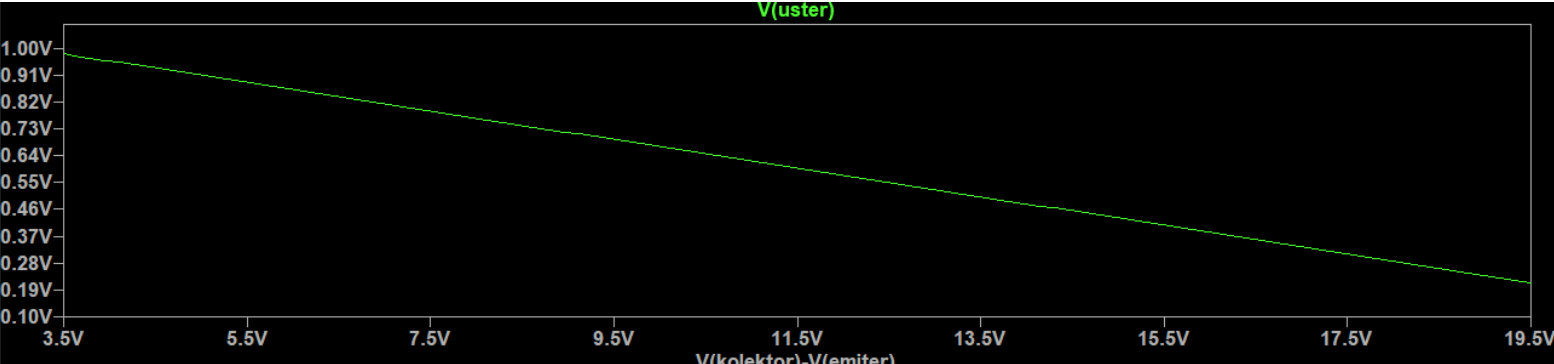
\includegraphics[scale=0.3]{p4.png}
    \centering
    \caption{$U_{strer}(U_{ce})$}
\end{figure}


\begin{figure}[h!]
    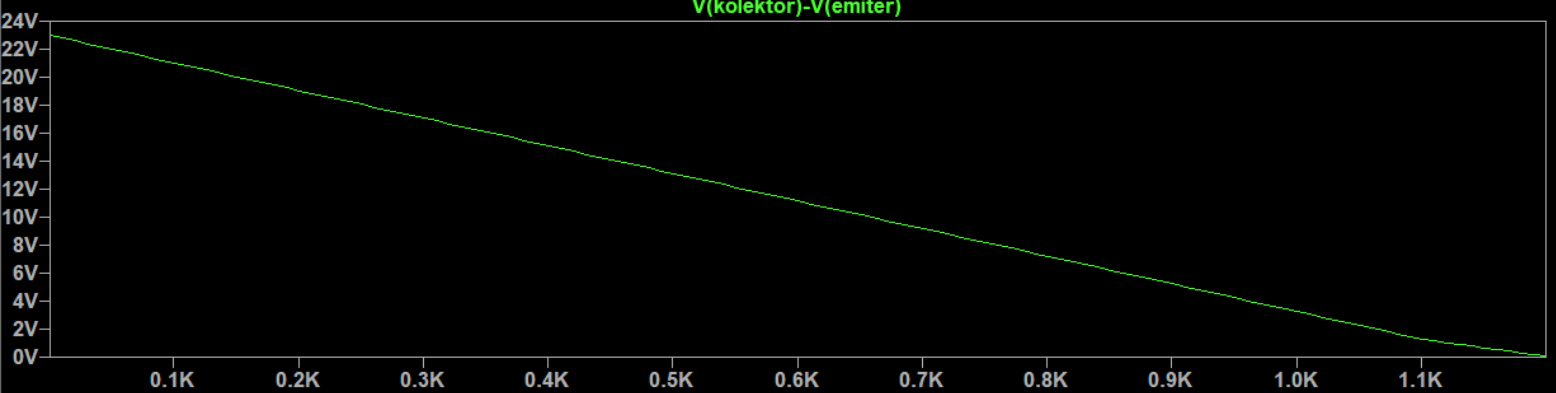
\includegraphics[scale=0.3]{p5.png}
    \centering
    \caption{$U_{ce}(R_{obc})$}
\end{figure}

\begin{figure}[h!]
    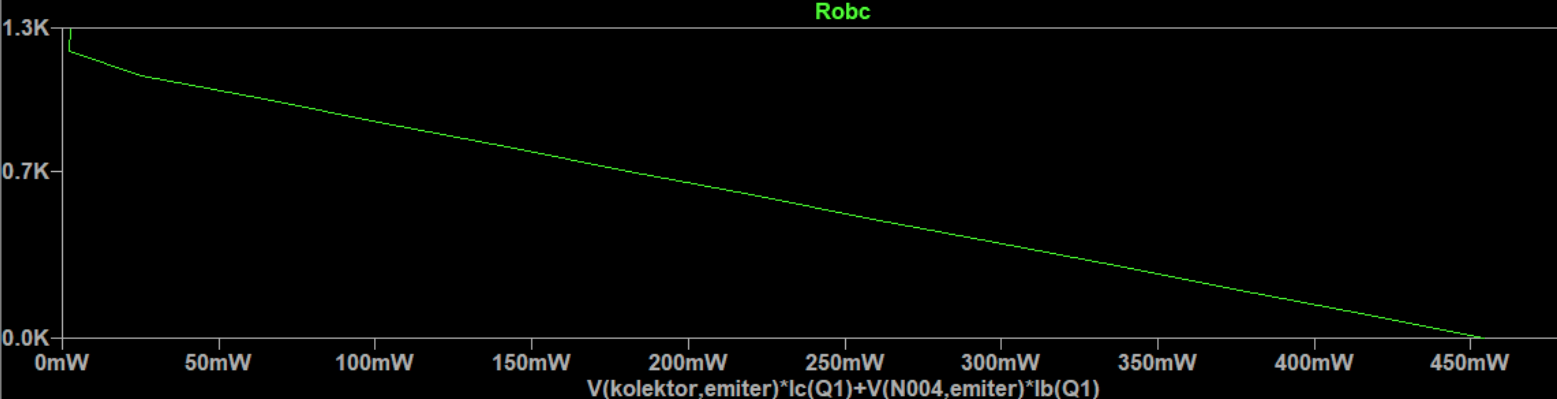
\includegraphics[scale=0.3]{p6.png}
    \centering
    \caption{$R_{obc}(P_{diss})$}
\end{figure}

\newpage
\subsection{$R_{pom}=250\Omega$}

Napięcia sterujące:\\
$U_{pom, 4mA}=4mA\cdot 250\Omega=1V$\\
$U_{pom, 20mA}=20mA\cdot 250\Omega=5V$


Dobranie rezystorów ($I_{1}=4mA$):


$$
    R_{1}=\frac{19V}{4mA}=4.75k\Omega
$$

$$
    R_{2}=\frac{1V}{4mA}250\Omega
$$

$$
    R_{ptn}=\frac{4V}{4mA}=1k\Omega
$$

Maksymalne wartości rezystancji obciążenia:

$$
    R_{MAX, 4ma}=\frac{24V-0.1V-1V}{4mA}=5725\Omega
$$

$$
    R_{MAX, 20mA}=\frac{24V-0.1V-5V}{20mA}=945\Omega
$$


\begin{figure}[h!]
    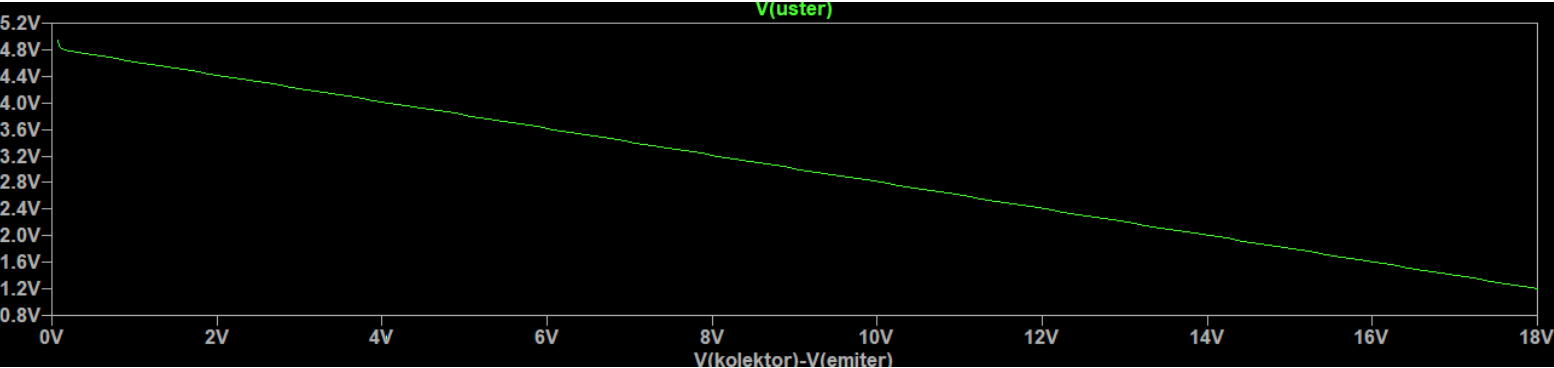
\includegraphics[scale=0.3]{p7.png}
    \centering
    \caption{$U_{strer}(U_{ce})$}
\end{figure}

\begin{figure}[h!]
    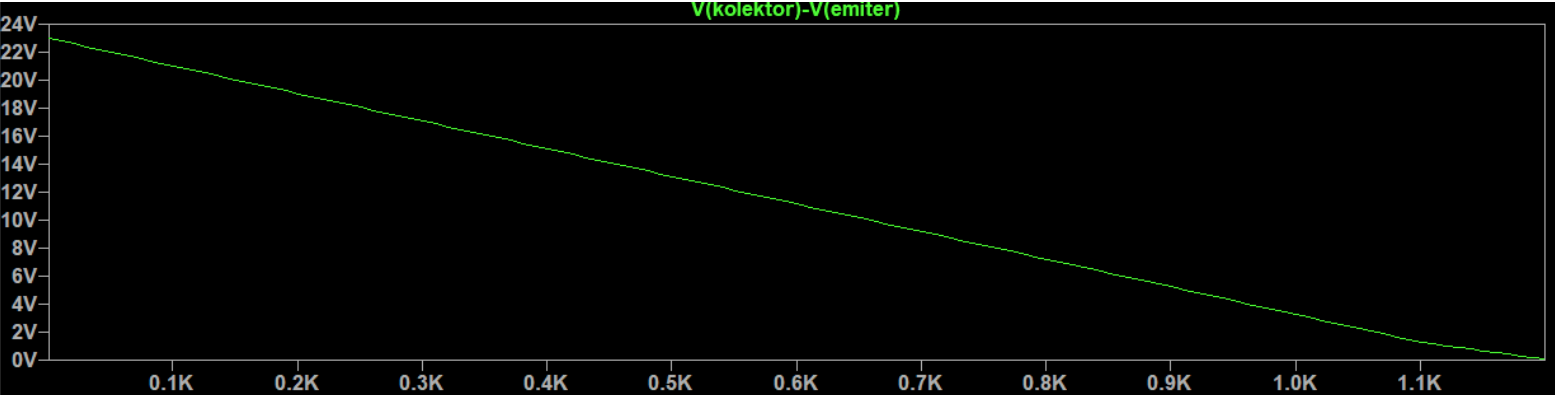
\includegraphics[scale=0.3]{p8.png}
    \centering
    \caption{$U_{ce}(R_{obc})$}
\end{figure}

\begin{figure}[h!]
    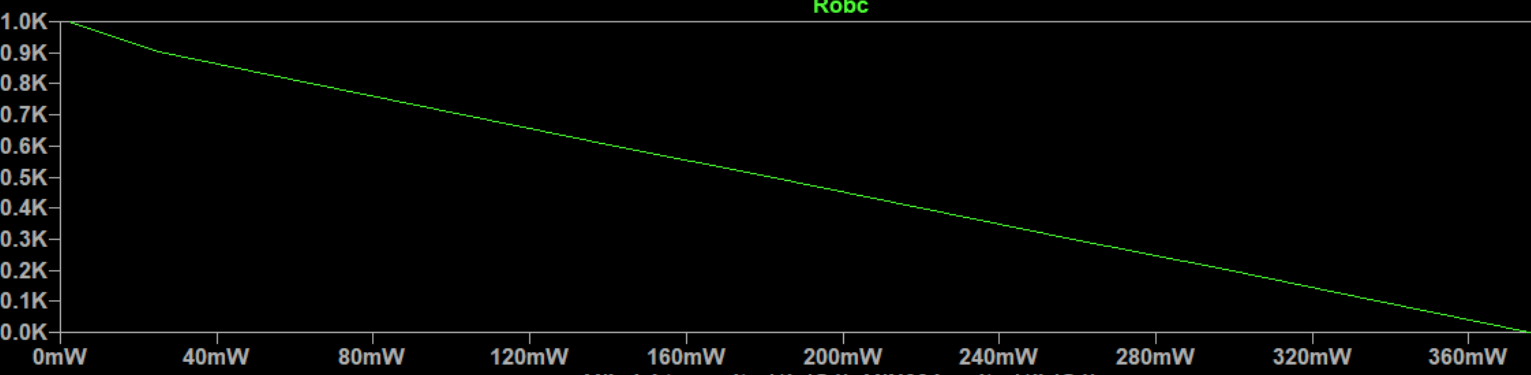
\includegraphics[scale=0.3]{p9.png}
    \centering
    \caption{$R_{obc}(P_{diss})$}
\end{figure}

\clearpage
\mbox{~}

\section{Moduł 4-20mA, Tranzystor PNP}

\begin{figure}[h!]
    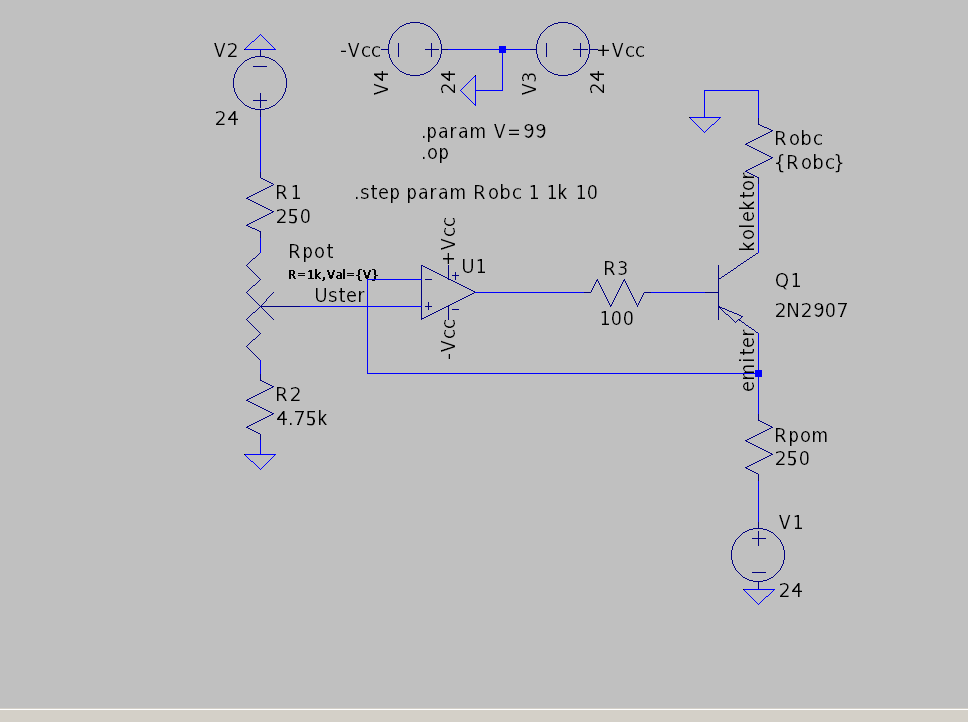
\includegraphics[scale=0.3]{schemat2.png}
    \caption{Układ z tranzystorem PNP}
\end{figure}

\subsection{$R_{pom}=10\Omega$}

Napięcia sterujące:\\
$U_{pom, 4mA}=24V-4mA\cdot 10\Omega=23.96V$\\
$U_{pom, 20mA}=24V-20mA\cdot 10\Omega=23.98V$

Dobranie rezystorów ($I_{1}=4mA$):

$$
    R_{1}=\frac{0.04V}{4mA}=10\Omega
$$

$$
    R_{2}=\frac{23.8V}{4mA}=5.95k\Omega
$$

$$
    R_{ptn}=\frac{0.16}{4mA}=40\Omega
$$

Maksymalne wartości rezystancji obciążenia:

$$
    R_{MAX, 4mA}=\frac{24V-0.1V-0.04V}{4mA}=5965\Omega
$$

$$
    R_{MAX, 20mA}=\frac{24V-0.1V-0.2V}{20mA}=1193\Omega
$$


\begin{figure}[h!]
    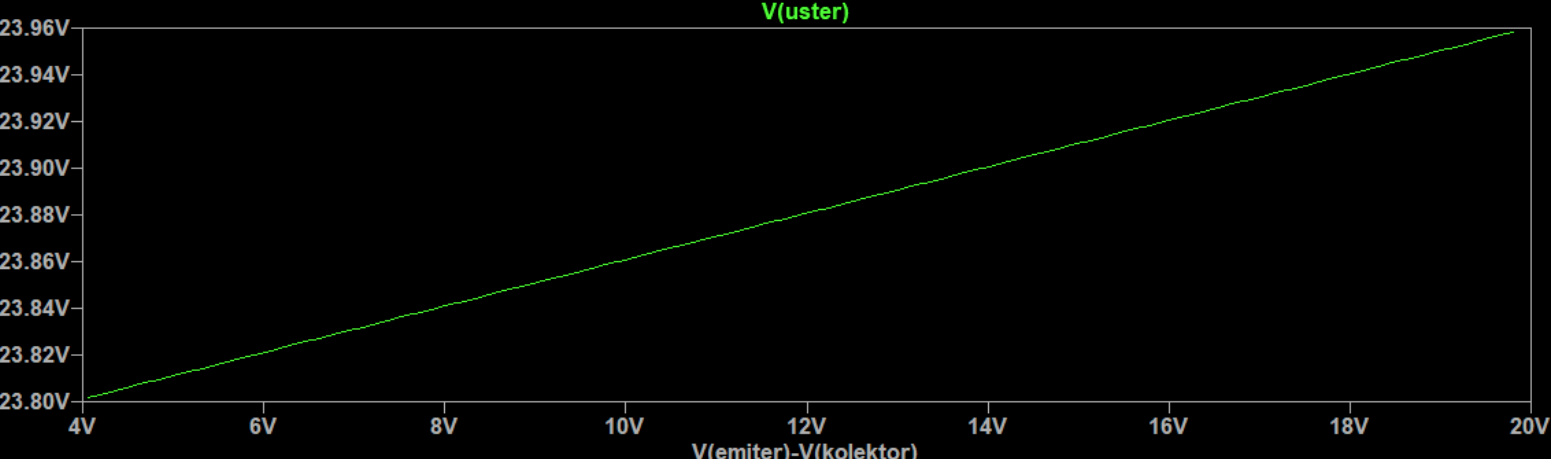
\includegraphics[scale=0.3]{p10.png}
    \centering
    \caption{$U_{strer}(U_{ce})$}
\end{figure}


\begin{figure}[h!]
    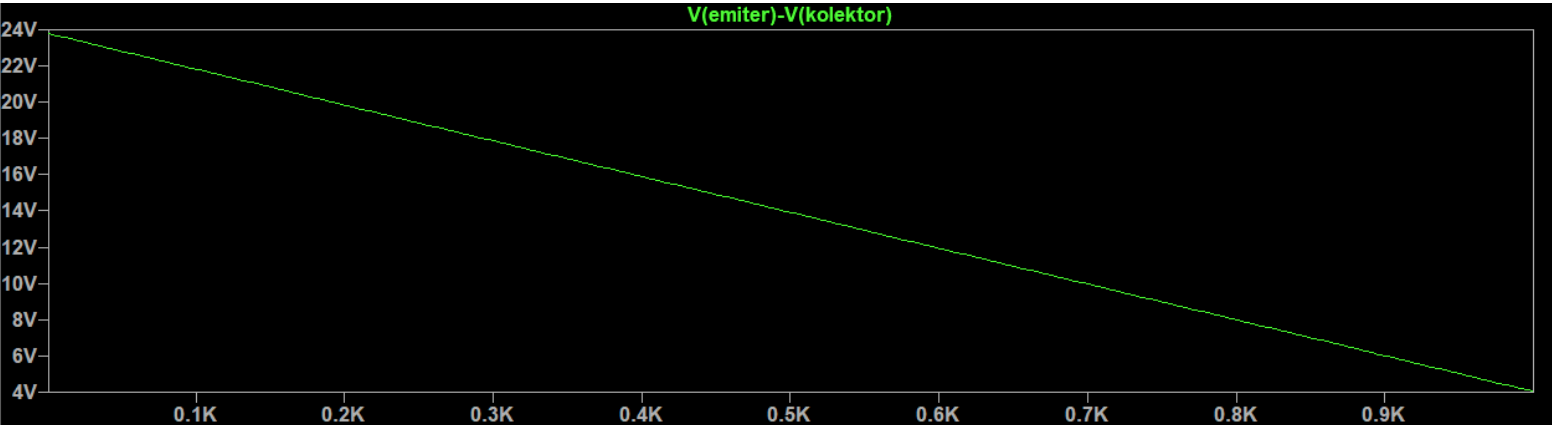
\includegraphics[scale=0.3]{p11.png}
    \centering
    \caption{$U_{ce}(R_{obc})$}
\end{figure}

\begin{figure}[h!]
    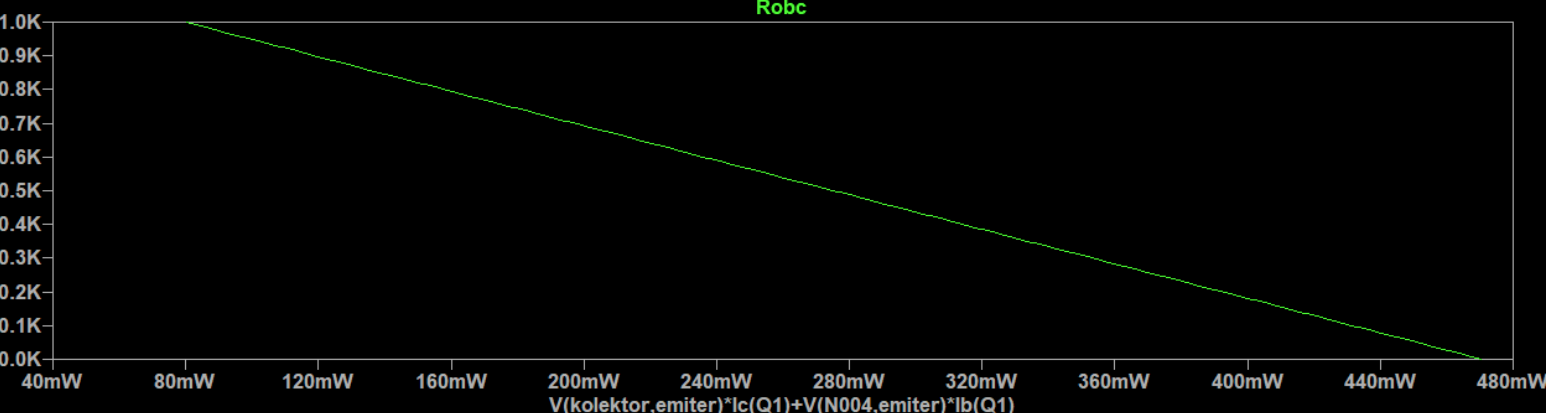
\includegraphics[scale=0.3]{p12.png}
    \centering
    \caption{$R_{obc}(P_{diss})$}
\end{figure}



\newpage


\subsection{$R_{pom}=50\Omega$}

Napięcia sterowania:\\
$U_{pom, 4mA}=24V-4mA\cdot 50\Omega=23.80V$\\
$U_{pom, 20mA}=24V-20mA\cdot 50\Omega=23V$


Dobranie rezystorów ($I_{1}=4mA$):

$$
    R_{1}=\frac{0.02V}{4mA}=50\Omega
$$

$$
    R_{2}=\frac{23V}{4mA}=5.75k\Omega
$$

$$
    R_{ptn}=\frac{0.8V}{4mA}=200\Omega
$$


Maksymalne wartości rezystancji obciążenia:

$$
    R_{MAX, 4mA}=\frac{24V-0.1V-0.2V}{4mA}=5925\Omega
$$

$$
    R_{MAX, 20mA}=\frac{24V-0.1V-1V}{20mA}=1145\Omega
$$


\begin{figure}[h!]
    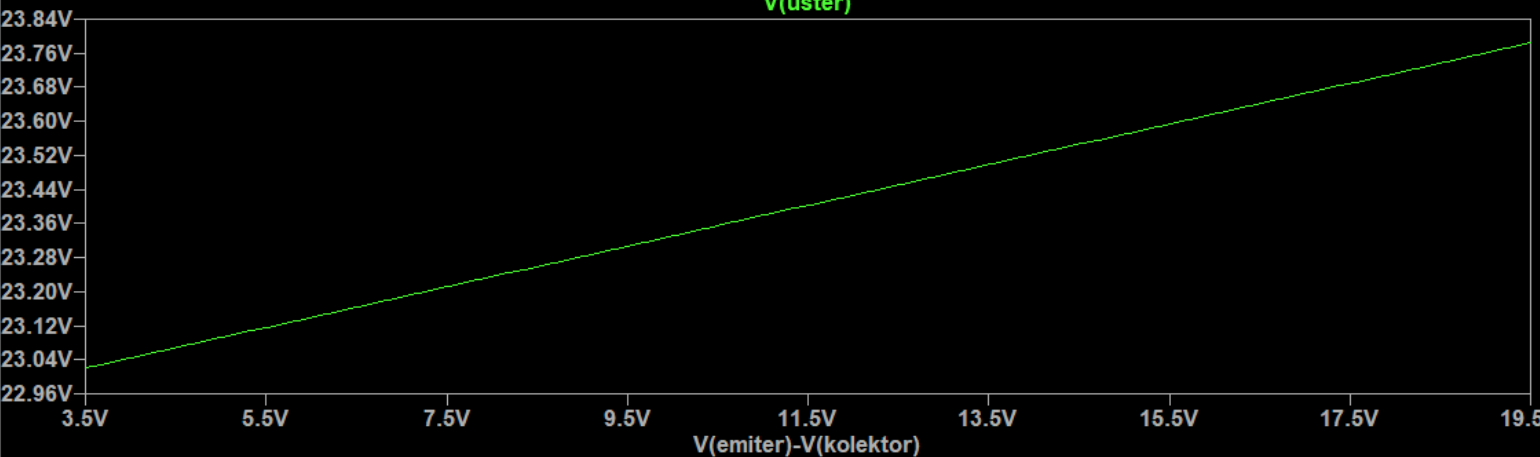
\includegraphics[scale=0.3]{p13.png}
    \centering
    \caption{$U_{strer}(U_{ce})$}
\end{figure}

\begin{figure}[h!]
    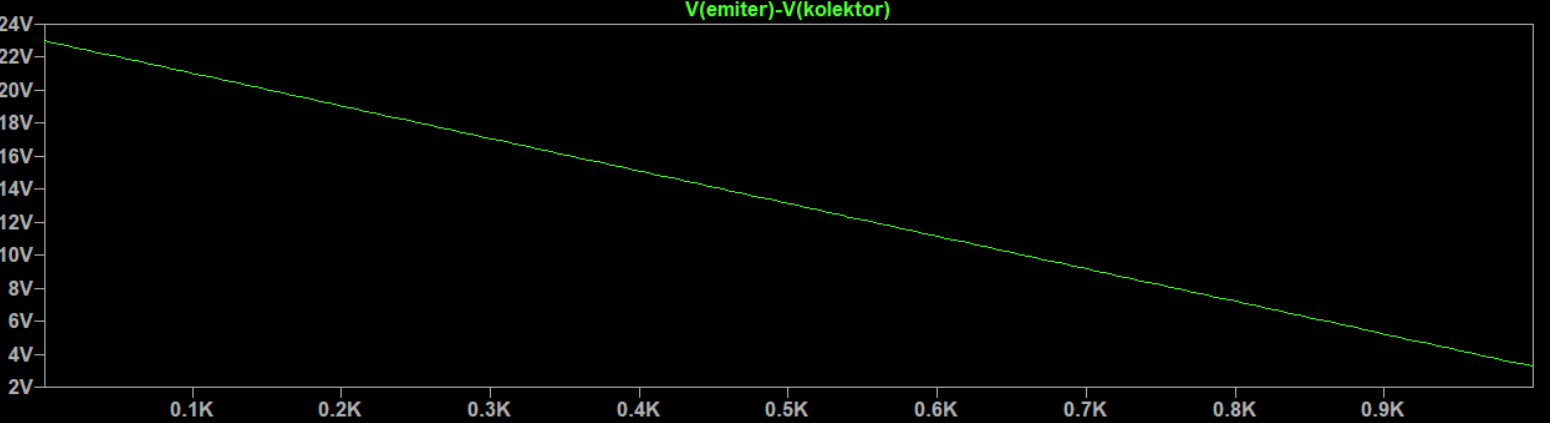
\includegraphics[scale=0.3]{p14.png}
    \centering
    \caption{$U_{ce}(R_{obc})$}
\end{figure}

\begin{figure}[h!]
    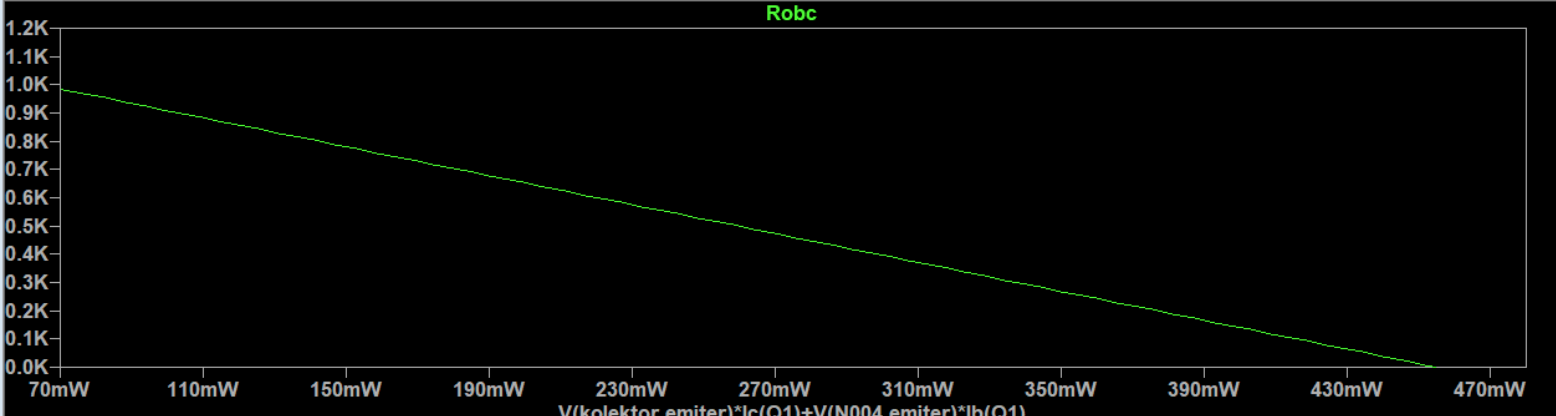
\includegraphics[scale=0.3]{p15.png}
    \centering
    \caption{$R_{obc}(P_{diss})$}
\end{figure}

\newpage

\subsection{$R_{pom}=250\Omega$}

Napięcia sterowania:\\
$U_{pom, 4mA}=24V-4mA\cdot 250\Omega=23V$\\
$U_{pom, 20mA}=24V-20mA\cdot 250\Omega=19V$

Dobranie rezystorów ($I_{1}=4mA$):

$$
    R_{1}=\frac{1V}{4mA}=250\Omega
$$

$$
    R_{2}=\frac{19V}{4mA}=4.75k\Omega
$$

$$
    R_{ptn}=\frac{4V}{4mA}=1k\Omega
$$


Maksymalne wartości rezystancji obciążenia:

$$
    R_{MAX, 4mA}=\frac{24V-0.1V-1V}{4mA}=5725\Omega
$$

$$
    R_{MAX, 20mA}=\frac{24V-0.1V-5V}{20mA}=945\Omega
$$


\begin{figure}[h!]
    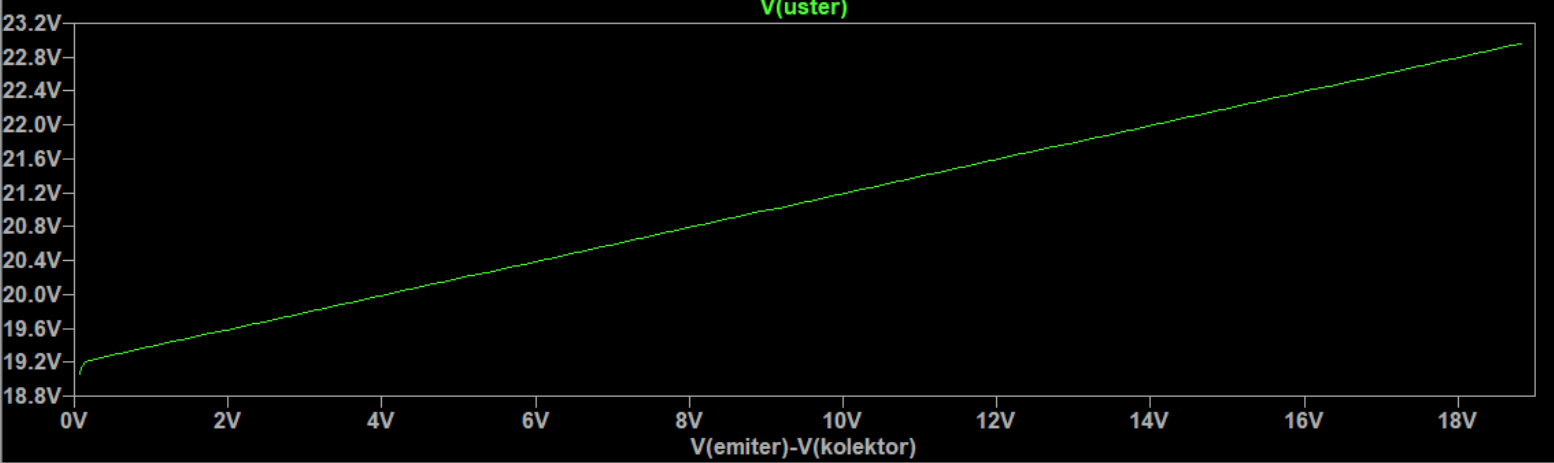
\includegraphics[scale=0.3]{p16.png}
    \centering
    \caption{$U_{strer}(U_{ce})$}
\end{figure}


\begin{figure}[h!]
    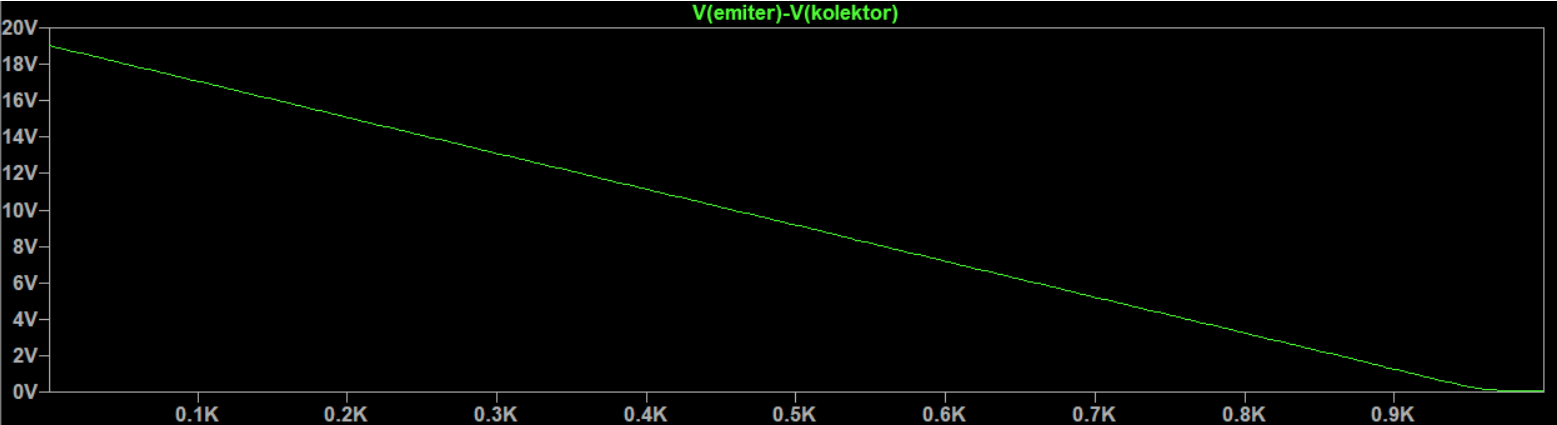
\includegraphics[scale=0.3]{p17.png}
    \centering
    \caption{$U_{ce}(R_{obc})$}
\end{figure}


\begin{figure}[h!]
    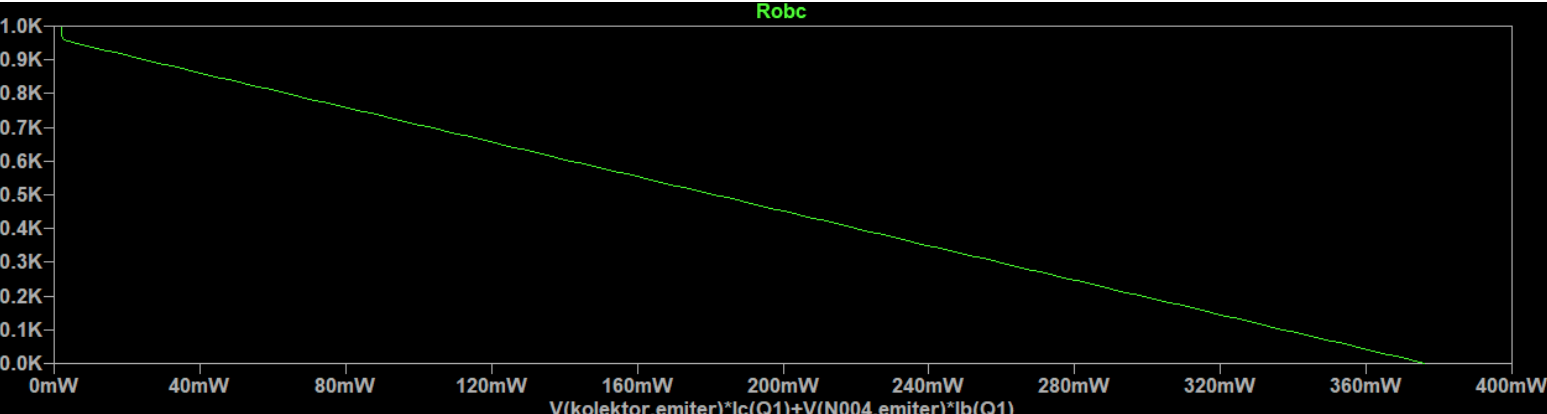
\includegraphics[scale=0.3]{p18.png}
    \centering
    \caption{$R_{obc}(P_{diss})$}
\end{figure}

\newpage

\section{Wnioski}

Układami z tranzystorami NPN można dobrze sterować na niższych napięciach niż układami z tranzystorami PNP. Maxymalne wartości rezystancji obciążenia dla $R_{pom}$ są identyczne dla układów z tranzystorem NPN i PNP, dlatego układy są symetryczne. Sterowanie potencjometrem jest odwrotne w zależności od użytego tranzystora.
\end{document}